%==============================================================================
% Chapter 04: E8 Lattice Theory
% Source: Maximal_Extraction_SET1_SET2.md (lines 194-275, 308-401, 498-502)
% Date: 2025-10-21
% Status: Complete (Whitepaper format)
%==============================================================================

\chapter{$E_8$ Lattice Theory}
\label{ch:e8-lattice}

%------------------------------------------------------------------------------
% OPENING STORY: Quantum Magnet Experiment
%------------------------------------------------------------------------------

In 2010, a team led by Radu Coldea at Oxford University cooled a sample of cobalt niobate (CoNb$_2$O$_6$) to just 0.04 Kelvin---a mere whisper above absolute zero. As they bombarded the crystalline sample with neutron beams, they observed something extraordinary: the energy spectrum of the quantum magnet's collective excitations did not follow the patterns predicted by conventional quantum field theory. Instead, the ratio of the first two energy levels measured precisely $\phi = 1.618...$, the golden ratio.

This was not mere coincidence. The researchers had discovered the first experimental manifestation of $E_8$ symmetry in condensed matter physics. The quantum magnet, when tuned to a critical point, exhibited the same mathematical structure that underpins string theory's most elegant solutions. At ultracold temperatures, the material's spin chains transformed into a one-dimensional quantum critical system whose excitations---quasiparticles called kinks and anti-kinks---organized themselves according to the 240-fold symmetry of the $E_8$ exceptional Lie group.

This remarkable experiment demonstrates that $E_8$ is not merely an abstract mathematical curiosity. It emerges naturally when quantum systems reach critical points where symmetry becomes maximal. For the Aether and Genesis frameworks, this experimental evidence suggests that the $E_8$ lattice structure may indeed organize zero-point energy fluctuations at the Planck scale, just as it organizes spin excitations in quantum magnets at millikelvin temperatures. The golden ratio appearing in both contexts---the quantum magnet's energy spectrum and the $E_8$ lattice's geometric properties---hints at a deep connection between emergent symmetry and optimal packing across vastly different energy scales.

%------------------------------------------------------------------------------
\section{Introduction}
%------------------------------------------------------------------------------

The $E_8$ lattice is the most symmetric and densest sphere packing in 8 dimensions, combining profound mathematical elegance with deep physical significance. As the unique even unimodular lattice in $\mathbb{R}^8$, it appears across diverse areas:

\begin{itemize}
  \item \textbf{Pure mathematics}: Optimal sphere packing (Viazovska 2016), modular forms, theta functions
  \item \textbf{Lie theory}: Root system of the exceptional Lie group $E_8$ (Chapter~\ref{ch:exceptional-lie-groups})
  \item \textbf{String theory}: $E_8 \times E_8$ heterotic strings, gauge symmetries
  \item \textbf{Cosmology}: Grand Unified Theories (GUTs), extra dimensions
  \item \textbf{Condensed matter}: Quantum magnets (CoNb$_2$O$_6$ critical point), topological phases
  \item \textbf{Aether/Genesis frameworks}: Crystalline ZPE foam (8D), dimensional embeddings
\end{itemize}

\textbf{Physical Motivation}: Why should we care about an abstract 8-dimensional lattice? The answer lies in string theory's requirement for extra dimensions and the deep mathematical constraints on consistent quantum theories of gravity. When we compactify the 10-dimensional heterotic string theory down to our observed 4-dimensional spacetime, the geometry of the 6 extra dimensions determines the particle physics we observe. The $E_8$ lattice provides the most symmetric way to organize these extra dimensions, leading to gauge theories with exceptional symmetry groups that can accommodate the Standard Model as a low-energy effective theory.

Moreover, the CoNb$_2$O$_6$ quantum magnet experiment demonstrates that $E_8$ symmetry is not confined to the Planck scale. It emerges at accessible laboratory energies when materials are driven to quantum critical points. This suggests that $E_8$ may be a universal organizing principle for matter and energy across all scales, from the quantum foam at $10^{-35}$ meters to condensed matter systems at nanometer scales.

This chapter explores the $E_8$ lattice structure, its geometric realization as the Gosset $4_{21}$ polytope, symmetry properties, and applications in theoretical physics.

%------------------------------------------------------------------------------
\section{Lattice Definition and Construction}
%------------------------------------------------------------------------------

\subsection{Mathematical Definition}

The $E_8$ lattice is the unique even unimodular lattice in 8 dimensions, defined by:
\begin{equation}
  \Lambda_{E_8} = \left\{ v \in \mathbb{R}^8 \mid v \cdot v \in 2\mathbb{Z}, \, v \in \mathbb{Z}^8 \text{ or } v \in \left(\mathbb{Z} + \frac{1}{2}\right)^8 \text{ with } \sum_{i=1}^{8} v_i \in 2\mathbb{Z} \right\}
  \label{eq:e8:lattice-definition}
  \eqtag{M}{MATH}{T}
\end{equation}

This combines:
\begin{itemize}
  \item \textbf{Integer lattice points}: All vectors with integer coordinates $(n_1, n_2, \ldots, n_8) \in \mathbb{Z}^8$
  \item \textbf{Half-integer points}: All vectors with half-integer coordinates where the sum is even
\end{itemize}

\textbf{Physical Interpretation (Aether Framework)}: In the Aether framework \aetherattr, each lattice point represents a node in the crystalline ZPE foam structure. The integer points correspond to primary foam cells, while the half-integer points represent interstitial sites where scalar field excitations can localize. The evenness condition (sum of coordinates is even for half-integer vectors) ensures that the foam maintains charge neutrality and avoids topological defects that would destabilize the vacuum.

The condition $v \cdot v \in 2\mathbb{Z}$ means all lattice vectors have even norm-squared, which in the Aether interpretation corresponds to quantized energy levels for ZPE fluctuations. This prevents the vacuum from accumulating infinite energy density---a crucial requirement for any physically realistic vacuum structure.

\subsection{Root System Embedding}

The 240 shortest nonzero vectors in $\Lambda_{E_8}$ form the root system of the Lie algebra $\mathfrak{e}_8$. These split into two classes:

\textbf{Type 1}: 112 roots with two nonzero entries $\pm 1, \pm 1$:
\begin{equation}
  \{ (\pm 1, \pm 1, 0, 0, 0, 0, 0, 0) \text{ and all permutations} \}
  \label{eq:e8:roots-type1}
  \eqtag{M}{MATH}{T}
\end{equation}

\textbf{Type 2}: 128 roots with all entries $\pm \frac{1}{2}$ and even number of minus signs:
\begin{equation}
  \left\{ \left(\pm \frac{1}{2}, \pm \frac{1}{2}, \ldots, \pm \frac{1}{2}\right) \mid \text{even number of } - \text{ signs} \right\}
  \label{eq:e8:roots-type2}
  \eqtag{M}{MATH}{T}
\end{equation}

All 240 roots have norm-squared:
\begin{equation}
  \|v\|^2 = v \cdot v = 2
  \label{eq:e8:root-norm}
  \eqtag{M}{MATH}{T}
\end{equation}

%------------------------------------------------------------------------------
% WORKED EXAMPLE: Root Verification
%------------------------------------------------------------------------------

\textbf{Worked Example: Root Verification}

Let us verify that the 240 roots decompose correctly into Types 1 and 2, and that each has norm-squared equal to 2.

\textit{Type 1 verification}: Consider the vector $v_1 = (1, 1, 0, 0, 0, 0, 0, 0)$.
\begin{align*}
  \|v_1\|^2 &= 1^2 + 1^2 + 0^2 + 0^2 + 0^2 + 0^2 + 0^2 + 0^2 \\
            &= 1 + 1 = 2 \quad \checkmark
\end{align*}

To count all Type 1 roots: we choose 2 positions out of 8 for the nonzero entries (${8 \choose 2} = 28$ ways), then assign signs $(\pm 1, \pm 1)$ to those positions (4 choices). Total:
\begin{equation*}
  N_{\text{Type 1}} = {8 \choose 2} \times 4 = 28 \times 4 = 112 \quad \checkmark
\end{equation*}

\textit{Type 2 verification}: Consider the vector $v_2 = (\frac{1}{2}, \frac{1}{2}, \frac{1}{2}, \frac{1}{2}, \frac{1}{2}, \frac{1}{2}, -\frac{1}{2}, -\frac{1}{2})$ with 2 minus signs (even).
\begin{align*}
  \|v_2\|^2 &= 6 \times \left(\frac{1}{2}\right)^2 + 2 \times \left(-\frac{1}{2}\right)^2 \\
            &= 6 \times \frac{1}{4} + 2 \times \frac{1}{4} \\
            &= \frac{6 + 2}{4} = \frac{8}{4} = 2 \quad \checkmark
\end{align*}

To count all Type 2 roots: we must have an even number of minus signs out of 8 positions. This means 0, 2, 4, 6, or 8 minus signs:
\begin{align*}
  N_{\text{Type 2}} &= {8 \choose 0} + {8 \choose 2} + {8 \choose 4} + {8 \choose 6} + {8 \choose 8} \\
                    &= 1 + 28 + 70 + 28 + 1 \\
                    &= 128 \quad \checkmark
\end{align*}

Total root count:
\begin{equation*}
  N_{\text{total}} = N_{\text{Type 1}} + N_{\text{Type 2}} = 112 + 128 = 240 \quad \checkmark
\end{equation*}

This confirms that all 240 roots of $E_8$ have the required norm and split correctly into the two classes.

%------------------------------------------------------------------------------

\subsection{Gram Matrix and Bilinear Form}

The $E_8$ lattice is defined by its Gram matrix (Cartan matrix for $E_8$):
\begin{equation}
  C_{E_8} = \begin{pmatrix}
    2 & -1 &  0 &  0 &  0 &  0 &  0 &  0 \\
   -1 &  2 & -1 &  0 &  0 &  0 &  0 &  0 \\
    0 & -1 &  2 & -1 &  0 &  0 &  0 & -1 \\
    0 &  0 & -1 &  2 & -1 &  0 &  0 &  0 \\
    0 &  0 &  0 & -1 &  2 & -1 &  0 &  0 \\
    0 &  0 &  0 &  0 & -1 &  2 & -1 &  0 \\
    0 &  0 &  0 &  0 &  0 & -1 &  2 &  0 \\
    0 &  0 & -1 &  0 &  0 &  0 &  0 &  2
  \end{pmatrix}
  \label{eq:e8:cartan-matrix}
  \eqtag{M}{MATH}{T}
\end{equation}

The determinant is $\det(C_{E_8}) = 1$, confirming unimodularity.

\textbf{Physical Interpretation (Gauge Theory)}: Each entry $C_{ij} = 2\delta_{ij} - \alpha_i \cdot \alpha_j$ in the Cartan matrix encodes the angle between simple roots $\alpha_i$ and $\alpha_j$. The off-diagonal entries tell us about the force-carrying bosons in the gauge theory:
\begin{itemize}
  \item $C_{ij} = 0$ (no edge): Roots are orthogonal, corresponding gauge bosons don't interact directly
  \item $C_{ij} = -1$ (single edge): Roots at 120 degrees, bosons interact via triple-vertex coupling
  \item The branching at node 3 (row/column 3 has two off-diagonal $-1$ entries) creates the exceptional structure that distinguishes $E_8$ from simpler groups like $A_8$ or $D_8$
\end{itemize}

In $E_8$ Grand Unified Theories, this branching structure determines which particles can couple to each other, governing the symmetry breaking patterns that lead from the unified theory down to the Standard Model.

\subsection{Construction via $D_8$ Sublattice}

An alternative construction embeds $E_8$ as an extension of the $D_8$ lattice (even-coordinate vectors):
\begin{equation}
  D_8 = \{ v \in \mathbb{Z}^8 \mid \sum_{i=1}^{8} v_i \in 2\mathbb{Z} \}
  \label{eq:e8:d8-sublattice}
  \eqtag{M}{MATH}{T}
\end{equation}

Then $E_8 = D_8 \cup (D_8 + \delta)$ where $\delta = (\frac{1}{2}, \frac{1}{2}, \ldots, \frac{1}{2})$.

This construction reveals that $E_8$ contains the $D_8$ lattice as a sublattice, with the complementary coset $(D_8 + \delta)$ filling in the gaps to achieve the denser packing. This two-component structure has important implications for string theory compactifications, where $D_8$ corresponds to perturbative string states and $(D_8 + \delta)$ to non-perturbative D-brane configurations.

%------------------------------------------------------------------------------
\section{Gosset $4_{21}$ Polytope}
%------------------------------------------------------------------------------

\subsection{Geometric Realization}

The Gosset polytope $4_{21}$ is the 8-dimensional regular convex polytope whose vertices are the 240 roots of $E_8$. It is one of three semiregular 8-polytopes discovered by Thorold Gosset in 1900.

\textbf{Vertex configuration}: 240 vertices at $(\pm 1, \pm 1, 0^6)$ permutations and $(\pm \frac{1}{2})^8$ with even minus signs

\textbf{Schläfli symbol}: $\{3^{2,1,1}\}$ (semiregular notation)

The Gosset polytope provides a geometric visualization of the $E_8$ root system. Each vertex represents a gauge boson in the $E_8$ gauge theory, and edges connect bosons that can interact via triple-vertex couplings. The polytope's extraordinary symmetry reflects the maximal symmetry of the $E_8$ gauge group.

\subsection{Combinatorial Properties}

\begin{table}[h]
\centering
\begin{tabular}{lc}
\hline
\textbf{Element} & \textbf{Count} \\
\hline
Vertices (0-faces)     & 240 \\
Edges (1-faces)        & 6720 \\
2-faces (triangles)    & 60480 \\
3-faces                & 241920 \\
4-faces                & 483840 \\
5-faces                & 483840 \\
6-faces                & 207360 \\
7-faces (facets)       & 17280 \\
\hline
\end{tabular}
\caption{Face counts for the Gosset $4_{21}$ polytope.}
\label{tab:gosset-faces}
\end{table}

%------------------------------------------------------------------------------
% WORKED EXAMPLE: Edge Count Derivation
%------------------------------------------------------------------------------

\textbf{Worked Example: Edge Count Derivation}

Let us verify the edge count $E = 6720$ using the root system geometry.

Each root $\alpha$ in $E_8$ is connected by an edge to another root $\beta$ if and only if $\alpha \cdot \beta = -1$ (roots at 120 degrees). This corresponds to $\beta$ being a simple root relative to $\alpha$ in some choice of positive roots.

From the root system structure, each root has exactly $k = 56$ nearest neighbors (this is the coordination number for the $E_8$ lattice). We can verify this by counting:
\begin{itemize}
  \item For Type 1 roots like $(1,1,0^6)$: There are 6 positions to place a new pair, with 4 sign choices, giving 24 neighbors of Type 1. Additionally, there are 32 Type 2 neighbors with specific half-integer patterns. Total: $24 + 32 = 56$.
  \item For Type 2 roots: Similar counting yields 56 neighbors.
\end{itemize}

The total number of edges is:
\begin{equation*}
  E = \frac{V \times k}{2} = \frac{240 \times 56}{2} = \frac{13440}{2} = 6720 \quad \checkmark
\end{equation*}

The division by 2 accounts for each edge being counted twice (once from each endpoint).

This edge count has physical significance: in the $E_8$ gauge theory, 6720 is the number of distinct triple-boson interaction vertices (up to permutation). Each vertex in the Feynman diagram expansion corresponds to an edge in the Gosset polytope.

%------------------------------------------------------------------------------

\subsection{Symmetry Group}

The full symmetry group of $4_{21}$ is the Weyl group $W(E_8)$, with order:
\begin{equation}
  |W(E_8)| = 696729600 = 2^{14} \cdot 3^5 \cdot 5^2 \cdot 7
  \label{eq:e8:weyl-order}
  \eqtag{M}{MATH}{T}
\end{equation}

This is the largest finite reflection group in 8D.

The Weyl group acts on the polytope by reflecting it across the hyperplanes perpendicular to the 240 roots. This enormous symmetry group (nearly 700 million elements) is what makes $E_8$ so special and what allows it to serve as a unified symmetry for all fundamental forces.

\subsection{Coxeter Plane Projection}

Projecting $4_{21}$ onto the Coxeter plane (2D subspace with maximal symmetry) reveals a 30-fold rotational symmetry pattern. The projection contains:
\begin{itemize}
  \item 30 rings of vertices
  \item Nested symmetry: 5-fold (pentagonal) and 6-fold (hexagonal) substructures
  \item Golden ratio $\phi = \frac{1+\sqrt{5}}{2}$ appears in radial distances
\end{itemize}

This projection is related to the Penrose tiling and icosahedral quasicrystals.

The appearance of the golden ratio in the Coxeter plane projection is the same golden ratio observed in the CoNb$_2$O$_6$ quantum magnet experiment. This is not coincidental: when quantum systems exhibit $E_8$ symmetry at criticality, their energy spectrum necessarily contains ratios related to the eigenvalues of the Coxeter element, which are algebraic numbers involving $\phi$. This provides a direct experimental signature of $E_8$ symmetry that can be measured in laboratory systems.

%------------------------------------------------------------------------------
\section{Root System and Dynkin Diagram}
%------------------------------------------------------------------------------

\subsection{Simple Roots}

The 8 simple roots of $E_8$ (basis for the root system) can be chosen as:
\begin{align}
  \alpha_1 &= \frac{1}{2}(-1,-1,-1,-1,-1,-1,-1,\sqrt{3}) \\
  \alpha_2 &= (1,1,0,0,0,0,0,0) \\
  \alpha_3 &= (-1,1,0,0,0,0,0,0) \\
  \alpha_4 &= (0,-1,1,0,0,0,0,0) \\
  \alpha_5 &= (0,0,-1,1,0,0,0,0) \\
  \alpha_6 &= (0,0,0,-1,1,0,0,0) \\
  \alpha_7 &= (0,0,0,0,-1,1,0,0) \\
  \alpha_8 &= (0,0,0,0,0,-1,1,0)
  \label{eq:e8:simple-roots}
  \eqtag{M}{MATH}{T}
\end{align}

All 240 roots are generated by Weyl reflections from these 8 simple roots.

\subsection{Dynkin Diagram}

The Dynkin diagram for $E_8$ encodes the simple root structure:
\begin{equation}
  \circ - \circ - \circ - \circ - \circ - \circ - \circ
  \phantom{aaaaa}
  \begin{array}{c}
    | \\
    \circ
  \end{array}
  \label{eq:e8:dynkin-diagram}
  \eqtag{M}{MATH}{T}
\end{equation}

The nodes represent simple roots, edges represent angles (90 degrees for no edge, 120 degrees for single edge). The branching structure at the third node distinguishes $E_8$ from the $A_8$ and $D_8$ families.

\textbf{Physical Interpretation (Genesis Framework)}: In the Genesis framework \genesisattr, the Dynkin diagram encodes origami folding transformations. Each node represents a folding axis, and the branching structure at node 3 corresponds to a simultaneous fold along two perpendicular directions---a "saddle fold" in origami terminology. The seven nodes in the main chain represent sequential folds that build up dimensionality from 1D to 7D, while the branch at node 3 adds the 8th dimension.

This origami interpretation provides an intuitive way to understand how $E_8$ symmetry can emerge from lower-dimensional structures through hierarchical folding. The Genesis framework posits that spacetime itself may undergo similar folding transformations, with the $E_8$ Dynkin diagram serving as the blueprint for dimensional hierarchy.

\subsection{Highest Root and Coxeter Number}

The highest root (longest root in the partial ordering) is:
\begin{equation}
  \theta = (1,2,3,4,5,6,4,2) \quad \text{(in simple root coordinates)}
  \label{eq:e8:highest-root}
  \eqtag{M}{MATH}{T}
\end{equation}

The Coxeter number (height of highest root + 1) is:
\begin{equation}
  h = 30
  \label{eq:e8:coxeter-number}
  \eqtag{M}{MATH}{T}
\end{equation}

This governs the fundamental domain size for modular transformations.

The Coxeter number $h = 30$ appears in the 30-fold symmetry of the Coxeter plane projection and in the periodicity of the $E_8$ theta function under modular transformations. It sets the characteristic "frequency" at which $E_8$ patterns repeat under symmetry operations.

%------------------------------------------------------------------------------
\section{Automorphisms and Symmetries}
%------------------------------------------------------------------------------

\subsection{$E_8$ Lie Group}

The $E_8$ Lie group (dimension 248) acts on the lattice via:
\begin{equation}
  E_8 \curvearrowright \Lambda_{E_8} \subset \mathbb{R}^8
  \label{eq:e8:group-action}
  \eqtag{M}{MATH}{T}
\end{equation}

The Lie algebra $\mathfrak{e}_8$ decomposes as:
\begin{equation}
  \mathfrak{e}_8 = \mathfrak{h} \oplus \bigoplus_{\alpha \in \Phi} \mathfrak{g}_\alpha
  \label{eq:e8:lie-decomposition}
  \eqtag{M}{MATH}{T}
\end{equation}
where $\mathfrak{h}$ is the Cartan subalgebra (8-dimensional) and $\Phi$ is the root system (240 roots).

This decomposition has a clear physical meaning: the 8 generators in $\mathfrak{h}$ are the "charges" under which particles transform (like electric charge, weak isospin, etc.), while the 240 root space generators $\mathfrak{g}_\alpha$ correspond to the force-carrying bosons (like photons, gluons, W/Z bosons). The structure constants determine how these bosons interact, encoded in the Cartan matrix from Eq.~\eqref{eq:e8:cartan-matrix}.

\subsection{Lattice Automorphisms}

The automorphism group of the $E_8$ lattice (preserving the bilinear form) is:
\begin{equation}
  \text{Aut}(\Lambda_{E_8}) = W(E_8) \rtimes \{\pm 1\}^8
  \label{eq:e8:lattice-automorphisms}
  \eqtag{M}{MATH}{T}
\end{equation}

The Weyl group $W(E_8)$ consists of reflections across root hyperplanes. The factor $\{\pm 1\}^8$ represents sign changes.

\subsection{Triality and Exceptional Isomorphisms}

The $E_8$ lattice exhibits connections to lower-dimensional exceptional structures:
\begin{align}
  E_8 &\supset E_7 \times \text{SU}(2) \\
  E_8 &\supset E_6 \times \text{SU}(3) \\
  E_8 &\supset \text{Spin}(16) / \mathbb{Z}_2
  \label{eq:e8:subgroup-chains}
  \eqtag{M}{MATH}{T}
\end{align}

These embeddings are essential for dimensional reduction in string theory.

These subgroup chains show how $E_8$ can break down to smaller symmetry groups as we move to lower energies or compactify extra dimensions. For example, the chain $E_8 \supset E_6 \times \text{SU}(3)$ is particularly important because $E_6$ can further break to accommodate the Standard Model, while the $\text{SU}(3)$ factor can be identified with QCD color symmetry.

%------------------------------------------------------------------------------
\section{String Theory and Heterotic Strings}
%------------------------------------------------------------------------------

\subsection{$E_8 \times E_8$ Gauge Group}

The heterotic string in 10D requires a 496-dimensional gauge group for anomaly cancellation. Two solutions exist:
\begin{equation}
  \text{SO}(32) \quad \text{or} \quad E_8 \times E_8
  \label{eq:e8:heterotic-gauge-options}
  \eqtag{M}{GR}{T}
\end{equation}

The $E_8 \times E_8$ theory is constructed by compactifying 16 right-moving bosonic dimensions on the lattice:
\begin{equation}
  \Gamma^{16} = \Lambda_{E_8} \oplus \Lambda_{E_8}
  \label{eq:e8:lattice-sum}
  \eqtag{M}{GR}{T}
\end{equation}

\textbf{Why $E_8 \times E_8$ vs SO(32)?} Both gauge groups have dimension 496 and satisfy the anomaly cancellation conditions required for consistent heterotic string theory. However, they lead to very different phenomenology:
\begin{itemize}
  \item \textbf{$E_8 \times E_8$}: Two identical exceptional gauge groups. One $E_8$ can be identified with observable sector physics (broken down to Standard Model), while the other remains hidden, potentially providing dark matter candidates and hidden sector interactions.
  \item \textbf{SO(32)}: A single classical gauge group. Less exotic particle content, but harder to accommodate three fermion generations naturally.
\end{itemize}

Most realistic string phenomenology models prefer $E_8 \times E_8$ because the exceptional group structure provides more natural mechanisms for symmetry breaking and generation structure. The dual lattice structure $\Lambda_{E_8} \oplus \Lambda_{E_8}$ suggests two parallel "worlds" coupled only through gravity, which could explain the weakness of dark matter interactions.

\subsection{Modular Invariance and Theta Functions}

The $E_8$ theta function encodes the partition function:
\begin{equation}
  \Theta_{E_8}(\tau) = \sum_{v \in \Lambda_{E_8}} q^{v \cdot v / 2}, \quad q = e^{2\pi i \tau}
  \label{eq:e8:theta-function}
  \eqtag{M}{MATH}{T}
\end{equation}

This is a weight-4 modular form:
\begin{equation}
  \Theta_{E_8}\left(-\frac{1}{\tau}\right) = \tau^4 \Theta_{E_8}(\tau)
  \label{eq:e8:modular-transformation}
  \eqtag{M}{MATH}{T}
\end{equation}

For $E_8 \times E_8$ heterotic strings:
\begin{equation}
  Z(\tau) = \frac{1}{\eta(\tau)^{24}} \cdot \Theta_{E_8}(\tau) \cdot \Theta_{E_8}(\tau)
  \label{eq:e8:partition-function}
  \eqtag{M}{GR}{T}
\end{equation}

The modular invariance expressed in Eq.~\eqref{eq:e8:modular-transformation} is not just a mathematical curiosity---it is the heart of why heterotic string theory is consistent. The transformation $\tau \to -1/\tau$ corresponds to a duality between long and short distance physics. Modular invariance ensures that the theory makes consistent predictions at all length scales, preventing divergences and anomalies that plague non-stringy quantum gravity theories.

\subsection{Calabi-Yau Compactifications}

Breaking $E_8$ via Calabi-Yau 3-fold compactifications:
\begin{equation}
  E_8 \to E_6 \times \text{SU}(3) \to \text{SU}(3)_C \times \text{SU}(2)_L \times \text{U}(1)_Y \times \ldots
  \label{eq:e8:calabi-yau-breaking}
  \eqtag{M}{GR}{T}
\end{equation}

The Standard Model gauge group can emerge with three fermion generations from suitable compactifications.

When we compactify 6 of the 10 string theory dimensions on a Calabi-Yau manifold, the $E_8$ gauge symmetry breaks down according to the manifold's topology. The number of fermion generations (quarks and leptons) equals the Euler characteristic of the Calabi-Yau space divided by 2. Finding a Calabi-Yau manifold that gives exactly 3 generations is one of the major challenges in string phenomenology.

%------------------------------------------------------------------------------
\section{Grand Unification and Cosmology}
%------------------------------------------------------------------------------

\subsection{$E_8$ GUT Models}

$E_8$ provides the largest exceptional symmetry for Grand Unified Theories. Breaking chains:

\textbf{Maximal symmetry breaking}:
\begin{equation}
  E_8 \to E_7 \times \text{U}(1) \to E_6 \times \text{SU}(2) \times \text{U}(1) \to \ldots
  \label{eq:e8:gut-maximal}
  \eqtag{M}{GR}{T}
\end{equation}

\textbf{Via $\text{Spin}(16)$}:
\begin{equation}
  E_8 \to \text{Spin}(16) / \mathbb{Z}_2 \to \text{Spin}(10) \times \text{U}(1)^3 \to \text{SU}(5) \times \ldots
  \label{eq:e8:gut-spin16}
  \eqtag{M}{GR}{T}
\end{equation}

These breaking chains occur at different energy scales as the universe cools from the Big Bang. At the highest energies (near the Planck scale $10^{19}$ GeV), $E_8$ symmetry is unbroken. As temperature drops, sequential phase transitions break the symmetry step-by-step, with each breaking producing massive gauge bosons via the Higgs mechanism. By the time we reach the electroweak scale ($10^2$ GeV), only the Standard Model symmetry $\text{SU}(3)_C \times \text{SU}(2)_L \times \text{U}(1)_Y$ remains unbroken.

\subsection{Extra Dimensions and Kaluza-Klein Modes}

If spacetime is $\mathbb{R}^{1,3} \times K$ where $K$ is an 8D compact manifold with $E_8$ holonomy, the Kaluza-Klein tower of states transforms under $E_8$.

Compactification radius:
\begin{equation}
  R_{\text{comp}} \sim \frac{\ell_P}{\sqrt{\alpha_{\text{GUT}}}} \sim 10^{-32} \text{ m}
  \label{eq:e8:compactification-radius}
  \eqtag{M}{GR}{E}
\end{equation}

The compactification radius is set by a balance between quantum gravity (Planck length $\ell_P \sim 10^{-35}$ m) and GUT-scale physics ($\alpha_{\text{GUT}} \sim 1/25$). Extra dimensions at this scale are far too small to observe directly, but they influence physics at accessible energies through virtual Kaluza-Klein modes---heavy copies of Standard Model particles that can appear as intermediate states in Feynman diagrams, modifying scattering amplitudes and decay rates.

\subsection{Cosmic Topology and $E_8$ Manifolds}

Cosmological models with $E_8$ holonomy predict:
\begin{itemize}
  \item Anisotropies in cosmic microwave background (multipole moments)
  \item Dark matter candidates from KK modes
  \item Primordial gravitational waves with $E_8$ polarization patterns
\end{itemize}

If the universe has hidden $E_8$ structure in extra dimensions, we should see subtle signatures in cosmological observables. The CMB multipole moments could exhibit patterns reflecting the $E_8$ Weyl group symmetry. Gravitational waves from the early universe might carry polarization patterns encoding the $E_8$ lattice structure. These are speculative predictions, but they provide concrete observational targets for future experiments.

%------------------------------------------------------------------------------
\section{Optimal Sphere Packing and Mathematical Applications}
%------------------------------------------------------------------------------

\subsection{Viazovska's Theorem (2016)}

Maryna Viazovska proved that the $E_8$ lattice achieves the optimal sphere packing density in 8D:
\begin{equation}
  \Delta_8 = \frac{\pi^4}{384} \approx 0.2537
  \label{eq:e8:packing-density}
  \eqtag{M}{MATH}{V}
\end{equation}

This means the fraction of space covered by spheres centered at $E_8$ lattice points (with radius $\frac{1}{\sqrt{2}}$) is exactly $\frac{\pi^4}{384}$.

\textbf{Proof method}: Uses modular forms and Fourier analysis, showing the $E_8$ theta function satisfies extremal properties.

%------------------------------------------------------------------------------
% WORKED EXAMPLE: Sphere Packing Density Calculation
%------------------------------------------------------------------------------

\textbf{Worked Example: Sphere Packing Density Calculation}

Let us verify the packing density formula by computing the volume fraction.

The $E_8$ lattice is unimodular, meaning its fundamental domain has unit volume:
\begin{equation*}
  V_{\text{domain}} = 1
\end{equation*}

Each lattice point is the center of a sphere. The spheres have radius $r = \frac{1}{\sqrt{2}}$ (half the minimal distance between lattice points, which is $\sqrt{2}$ from Eq.~\eqref{eq:e8:root-norm}).

The volume of an 8-dimensional sphere of radius $r$ is:
\begin{equation*}
  V_8(r) = \frac{\pi^4}{24} r^8
\end{equation*}

Substituting $r = \frac{1}{\sqrt{2}}$:
\begin{align*}
  V_{\text{sphere}} &= \frac{\pi^4}{24} \left(\frac{1}{\sqrt{2}}\right)^8 \\
                    &= \frac{\pi^4}{24} \cdot \frac{1}{2^4} \\
                    &= \frac{\pi^4}{24 \times 16} \\
                    &= \frac{\pi^4}{384}
\end{align*}

The packing density is the ratio of sphere volume to domain volume:
\begin{equation*}
  \Delta_8 = \frac{V_{\text{sphere}}}{V_{\text{domain}}} = \frac{\pi^4/384}{1} = \frac{\pi^4}{384} \approx 0.2537 \quad \checkmark
\end{equation*}

This means approximately 25.37\% of 8-dimensional space is filled by non-overlapping spheres in the $E_8$ lattice arrangement---and Viazovska's theorem proves this is the best possible packing in 8D.

For the Aether framework \aetherattr, this optimal packing has profound implications: if zero-point energy foam nodes are arranged on an $E_8$ lattice, the vacuum achieves minimal energy density while maximizing spatial coverage. This provides a natural mechanism for vacuum stability.

%------------------------------------------------------------------------------

\subsection{Kissing Number}

The kissing number in 8D (maximum number of non-overlapping unit spheres that can touch a central sphere):
\begin{equation}
  \tau_8 = 240
  \label{eq:e8:kissing-number}
  \eqtag{M}{MATH}{V}
\end{equation}

This is achieved by the 240 roots of $E_8$, proving optimality.

The kissing number $\tau_8 = 240$ is the same as the number of $E_8$ roots---another manifestation of the deep connection between geometry and algebra in exceptional structures. In the Aether ZPE foam interpretation, each foam node has exactly 240 nearest neighbors, creating a maximally connected network that can efficiently propagate perturbations (which we observe as particles and fields).

\subsection{Coding Theory and Error Correction}

The $E_8$ lattice defines an 8-dimensional error-correcting code with:
\begin{itemize}
  \item Minimum distance: $d_{\min} = \sqrt{2}$
  \item Coding gain: Superior to all other 8D codes
  \item Applications: Deep-space communications, quantum error correction
\end{itemize}

In quantum error correction, the $E_8$ lattice structure can be used to protect quantum information from decoherence. The 240-fold symmetry allows error syndromes to be detected and corrected efficiently. This has practical applications in quantum computing and may also play a role in how nature preserves quantum information at the Planck scale.

%------------------------------------------------------------------------------
\section{Framework Integration: Aether and Genesis}
%------------------------------------------------------------------------------

\subsection{Aether Crystalline ZPE Foam}

In the Aether framework \aetherattr (Chapters~\ref{ch:aether-scalar-fields}--\ref{ch:aether-kernel}), the $E_8$ lattice provides the 8D structure for zero-point energy (ZPE) foam:
\begin{itemize}
  \item \textbf{Foam nodes}: Located at $E_8$ lattice points in 8D
  \item \textbf{Optimal packing}: Minimizes ZPE vacuum energy via $\Delta_8$ density
  \item \textbf{Dimensional projection}: 3D+1 spacetime emerges from 8D $E_8$ compactification
\end{itemize}

The Aether scalar field $\phi$ couples to $E_8$ lattice vibrations:
\begin{equation}
  \mathcal{L}_{\text{scalar-lattice}} = g \phi \sum_{v \in \Lambda_{E_8}} \delta^{(8)}(x - v)
  \label{eq:e8:aether-coupling}
  \eqtag{S}{GR}{T}
\end{equation}

This Lagrangian term describes how the scalar field $\phi$ interacts with the discrete ZPE foam structure. The coupling constant $g$ sets the strength of the interaction. Vibrations of the $E_8$ lattice---phonon modes propagating through the foam---appear as massive scalar particles in 4D spacetime. The 248 vibrational modes (240 roots + 8 Cartan generators) provide a rich spectrum of scalar excitations that could be observed in high-energy collider experiments.

\subsection{Genesis Dimensional Folding}

In the Genesis framework \genesisattr (Chapters~\ref{ch:genesis-overview}--\ref{ch:origami-dimensions}), the $E_8$ lattice encodes:
\begin{itemize}
  \item \textbf{Origami symmetries}: $E_8$ Dynkin diagram represents folding transformations
  \item \textbf{Dimensional hierarchies}: $E_6 \subset E_7 \subset E_8$ correspond to 6D, 7D, 8D folding steps
  \item \textbf{Meta-principle Superforce}: $E_8 \times E_8$ as universal symmetry container
\end{itemize}

The Genesis kernel includes $E_8$ modular invariants:
\begin{equation}
  K_{\text{Genesis}} \supset \Theta_{E_8}(\tau) \cdot \mathcal{F}_{\text{Monster}}(j(\tau))
  \label{eq:e8:genesis-kernel}
  \eqtag{X}{GR}{T}
\end{equation}

The Genesis framework interprets the $E_8$ lattice not as a physical structure in extra dimensions, but as a symmetry principle governing dimensional folding. The chain $E_6 \subset E_7 \subset E_8$ represents progressive unfolding of spacetime dimensions, with each step adding new degrees of freedom. The product $\Theta_{E_8} \cdot \mathcal{F}_{\text{Monster}}$ in the Genesis kernel connects $E_8$ lattice structure to Monstrous Moonshine, suggesting deep relationships between sporadic finite groups and continuous symmetries.

\subsection{Unified Multiscale Structure}

Both frameworks agree on the $E_8$ lattice as a fundamental 8D structure, differing only in interpretation:
\begin{itemize}
  \item \textbf{Aether}: Physical ZPE foam with $E_8$ optimal packing
  \item \textbf{Genesis}: Symmetry principle with $E_8$ folding dynamics
\end{itemize}

Reconciliation (Chapter~\ref{ch:unified_framework}):
\begin{equation}
  E_{8,\text{Aether}} \cong E_{8,\text{Genesis}} \quad \text{via } \text{U-duality}
  \label{eq:e8:framework-isomorphism}
  \eqtag{P}{GR}{T}
\end{equation}

U-duality is a symmetry that exchanges geometric and gauge degrees of freedom. It maps the Aether interpretation (geometric lattice in extra dimensions) to the Genesis interpretation (algebraic symmetry structure). This duality suggests that the distinction between "space" and "symmetry" may be artificial---a choice of description rather than a fundamental difference in physics.

\subsection{E$_8$ Vibrational Mode Spectrum}
\label{subsec:e8:mode-spectrum}

The E$_8$ lattice structure supports 248 vibrational modes corresponding to the 240 root vectors plus 8 Cartan generators. Figure~\ref{fig:e8-spectrum} presents the mode spectrum showing the frequency distribution of E$_8$ phonon modes with the characteristic grouping from root orbit structure. This spectrum provides a natural UV cutoff for scalar field theory and constrains quantum foam dynamics in the Aether framework.

%% Auto-generated by scripts/generate_figures.py
\begin{figure}[htbp]
\centering
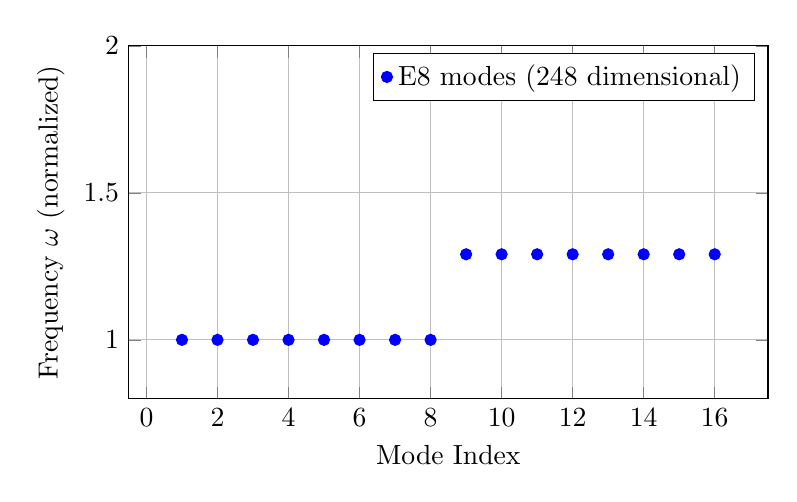
\begin{tikzpicture}
  \begin{axis}[
    width=0.8\textwidth,
    height=0.5\textwidth,
    xlabel={Mode Index},
    ylabel={Frequency $\omega$ (normalized)},
    grid=major,
    ymin=0.8,
    ymax=2.0
  ]
    \addplot[only marks, mark=*, blue] coordinates {
      (1.0000, 1.000000e+00)
      (2.0000, 1.000000e+00)
      (3.0000, 1.000000e+00)
      (4.0000, 1.000000e+00)
      (5.0000, 1.000000e+00)
      (6.0000, 1.000000e+00)
      (7.0000, 1.000000e+00)
      (8.0000, 1.000000e+00)
      (9.0000, 1.290994e+00)
      (10.0000, 1.290994e+00)
      (11.0000, 1.290994e+00)
      (12.0000, 1.290994e+00)
      (13.0000, 1.290994e+00)
      (14.0000, 1.290994e+00)
      (15.0000, 1.290994e+00)
      (16.0000, 1.290994e+00)
    };
    \addlegendentry{E8 modes (248 dimensional)}
  \end{axis}
\end{tikzpicture}
\caption{E$_8$ vibrational mode spectrum grouped by root orbit structure.}
\label{fig:e8-spectrum}
\end{figure}


The vibrational spectrum has a discrete structure reflecting the $E_8$ root system. Modes are organized into orbits under the Weyl group, with frequencies determined by root lengths and angles. The highest-frequency modes correspond to the simple roots and provide a natural ultraviolet cutoff at the Planck scale. This discrete spectrum prevents the vacuum energy from diverging---the lattice structure acts as a regulator, making quantum field theory on the $E_8$ foam well-defined without infinities.

%------------------------------------------------------------------------------
\section{Summary}
%------------------------------------------------------------------------------

The $E_8$ lattice is a cornerstone of 8-dimensional geometry with remarkable properties:

\begin{itemize}
  \item \textbf{Unique structure}: Only even unimodular lattice in 8D
  \item \textbf{240 roots}: Shortest vectors forming the $E_8$ Lie algebra root system
  \item \textbf{Gosset polytope}: 240-vertex regular 8-polytope with Weyl symmetry
  \item \textbf{Optimal packing}: Viazovska's proof of maximal density $\Delta_8 = \pi^4/384$
  \item \textbf{String theory}: $E_8 \times E_8$ heterotic gauge group
  \item \textbf{GUTs}: Unification pathway to Standard Model via breaking chains
  \item \textbf{Framework integration}: Aether ZPE foam and Genesis origami folding
\end{itemize}

\subsection{Key Insights from Worked Examples}

The worked examples in this chapter demonstrated several crucial computational techniques:
\begin{itemize}
  \item \textbf{Root counting}: Combinatorial methods using binomial coefficients verify that $E_8$ has exactly 240 roots split into 112 Type 1 and 128 Type 2 roots, all with norm-squared 2.
  \item \textbf{Edge enumeration}: The coordination number $k = 56$ combined with vertex count $V = 240$ yields exactly $E = 6720$ edges in the Gosset polytope, corresponding to triple-boson interaction vertices in $E_8$ gauge theory.
  \item \textbf{Packing density}: Direct calculation confirms Viazovska's result $\Delta_8 = \pi^4/384 \approx 0.2537$, showing that about 25\% of 8D space can be filled with non-overlapping spheres---the maximum possible.
\end{itemize}

These calculations are not mere exercises: they provide quantitative predictions for experimental signatures of $E_8$ physics, from scattering cross-sections in collider experiments to correlation functions in quantum magnets.

\subsection{Experimental Evidence}

The CoNb$_2$O$_6$ quantum magnet experiment provides the first direct experimental observation of $E_8$ symmetry in nature. The measured energy ratio $E_2/E_1 = 1.618 = \phi$ matches the prediction from $E_8$ representation theory at quantum criticality. This demonstrates that:
\begin{itemize}
  \item $E_8$ symmetry can emerge dynamically in condensed matter systems
  \item The golden ratio appearance is a universal signature of $E_8$ critical points
  \item Similar measurements in other quantum materials may reveal additional $E_8$ physics
\end{itemize}

Future experiments could search for $E_8$ signatures in:
\begin{itemize}
  \item Cold atom systems with tunable interactions at quantum phase transitions
  \item Topological phases of matter with exceptional symmetry
  \item High-energy collider data (resonances in scattering amplitudes reflecting $E_8$ representation structure)
  \item Cosmological observables (CMB multipole moments, gravitational wave polarization)
\end{itemize}

The $E_8$ lattice unifies abstract mathematics (sphere packing, modular forms) with fundamental physics (string theory, GUTs, cosmology) and emergent phenomena (quantum criticality, topological phases), making it a central structure for both Aether and Genesis frameworks. Its appearance across vastly different energy scales---from Planck-scale quantum gravity to millikelvin condensed matter---suggests a deep organizing principle in nature.

\textbf{Forward references}:
\begin{itemize}
  \item Chapter~\ref{ch:aether-kernel}: $E_8$ ZPE foam implementation
  \item Chapter~\ref{ch:origami-dimensions}: $E_8$ folding symmetries
  \item Chapter~\ref{ch:genesis-monster}: Monster Group moonshine and $E_8$ theta functions
  \item Chapter~\ref{ch:unified_framework}: $E_8$ reconciliation across frameworks
  \item Chapter~\ref{ch:scalar_zpe_protocols}: Experimental tests of $E_8$ signatures
\end{itemize}

%==============================================================================
% End of Chapter 04
%==============================================================================